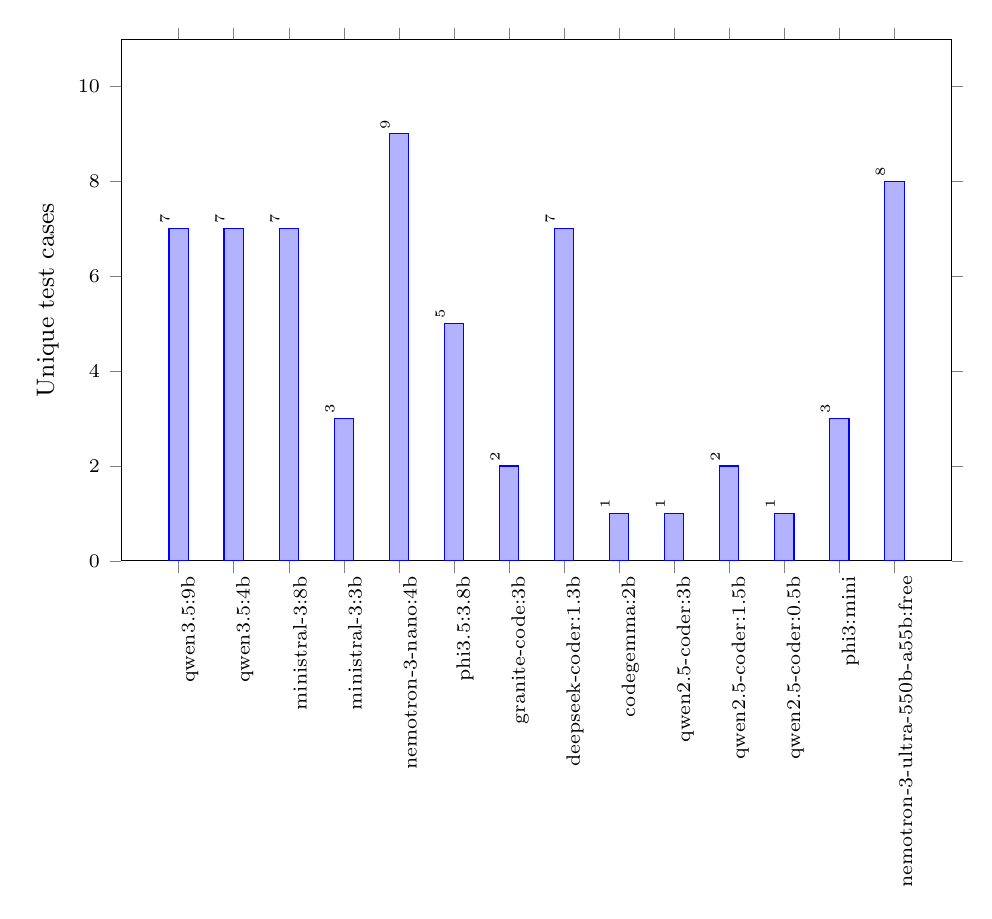
\begin{tikzpicture}
\begin{axis}[
  ybar,
  bar width=7pt,
  bar shift=0pt,
  width=\textwidth,
  height=8.2cm,
  ylabel={Unique test cases},
  xtick={0,1,2,3,4,5,6,7,8,9,10,11,12,13},
  xticklabels={qwen3.5:9b,qwen3.5:4b,ministral-3:8b,ministral-3:3b,nemotron-3-nano:4b,phi3.5:3.8b,granite-code:3b,deepseek-coder:1.3b,codegemma:2b,qwen2.5-coder:3b,qwen2.5-coder:1.5b,qwen2.5-coder:0.5b,phi3:mini,nemotron-3-ultra-550b-a55b:free},
  x tick label style={rotate=90, anchor=east, font=\scriptsize, inner sep=1pt, yshift=-4pt},
  y tick label style={font=\scriptsize},
  label style={font=\small},
  ymin=0,
  ymax=10.980000,
  enlarge x limits=0.08,
  tick align=outside,
  clip=false,
]
\addplot+[bar shift=0pt] coordinates {(0,7.000000) (1,7.000000) (2,7.000000) (3,3.000000) (4,9.000000) (5,5.000000) (6,2.000000) (7,7.000000) (8,1.000000) (9,1.000000) (10,2.000000) (11,1.000000) (12,3.000000) (13,8.000000)};
\addplot[
  only marks,
  mark=none,
  bar shift=0pt,
  forget plot,
  nodes near coords,
  point meta=explicit symbolic,
  every node near coord/.append style={font=\tiny, rotate=90, anchor=west, inner sep=1.5pt, yshift=5pt, fill=white, fill opacity=0.9, text opacity=1},
] table[x=x,y=y,meta=label] {
x y label
0 7.000000 {7}
1 7.000000 {7}
2 7.000000 {7}
3 3.000000 {3}
4 9.000000 {9}
5 5.000000 {5}
6 2.000000 {2}
7 7.000000 {7}
8 1.000000 {1}
9 1.000000 {1}
10 2.000000 {2}
11 1.000000 {1}
12 3.000000 {3}
13 8.000000 {8}
};
\end{axis}
\end{tikzpicture}
